\chapter{How to Write Descriptively}

This lecture begins from the reader's side and only then turns toward craft. We ask first why fiction matters, then what prose must do if it is to absorb us as strongly as lived experience, theater, or film. The central claim is that descriptive language is not ornament laid over a story. It is one of the mechanisms by which static marks on a page become sensation, association, and finally immersion.

\section{Why We Read Fiction, and What Description Must Achieve}

The opening list is deliberately wide. We read fiction to be entertained, to discover what happened, to travel, to fear, to laugh, to cry, to think, and to feel. But the lecture does not stop at a catalog of pleasures. It ends that list at the strongest point: we read to become so absorbed that, for a time, we forget where we are. This gives the lecture its governing relation,
\begin{equation}
\text{fiction} \Rightarrow \text{absorption / immersion}.
\end{equation}

\begin{definition}
Immersion is the temporary spell in which the reader is not merely informed about a story world but feels present within it.
\end{definition}

Once that standard is fixed, the lecturer can turn the problem around. If this is what fiction must do for us, how does a writer accomplish it? The lecture names the obvious candidates and weighs them quickly:
\begin{equation}
\text{reader engagement} \leftarrow \{\text{plot},\ \text{character},\ \text{language}\}.
\end{equation}
Plot may help. Character probably helps. Beautiful language perhaps helps. The word ``perhaps'' is important, because it opens the door to the real subject of the lecture. We are about to ask what kind of language does the work.

\subsection{Question \& Answer}

\paragraph{Question.} What does fiction have to do on the page if it wants to hold us?

\paragraph{Answer.} It must do more than tell us what happened. It must induce a state in which the reader is imaginatively relocated into the story. The lecture begins with that demand so that every later craft claim can be measured against it.

\section{Metaphor Against Statement: The Billy Example}

The first serious test comes immediately. We are given a description: Billy's legs are noodles; the ends of her hair are poison needles; her tongue is a bristly sponge; her eyes are bags of bleach. Then the lecturer asks a sharp question: did that almost make us feel as queasy as Billy? The answer is no, not completely. Yet we are still closer to Billy's condition than we would be if the sentence simply reported that she felt nauseated and weak.

That local contrast can be compressed as
\begin{equation}
\text{metaphorical description} > \text{flat paraphrase},
\end{equation}
where the symbol \(>\) does not mean numerical magnitude. It means greater vividness, greater pressure on the senses, and therefore a better chance of moving from knowledge toward feeling.

The lecture is careful here. Billy's legs are not literally noodles. The point is not confusion but implied comparison. The metaphor works because it translates an internal state into bodily terms that the reader can partially simulate. Once we replace that phrasing with summary, the sensory bridge collapses. We still understand, but we do not experience the condition in the same way. This is the first real theorem of the chapter:
\begin{equation}
\text{understanding} \neq \text{feeling}, \qquad
\text{reading} \neq \text{immersion}.
\end{equation}

\subsection{Question \& Answer}

\paragraph{Question.} Why does the metaphorical version feel stronger than the literal paraphrase?

\paragraph{Answer.} Because the metaphor does not merely classify Billy's state; it re-encodes that state in sensory terms. The paraphrase gives us diagnosis. The metaphor gives us a way to inhabit the diagnosis.

\section{Prose as Static Symbols, and the Construction of Experience}

At this point the lecture enlarges its claim. The point of fiction, we are told, is to cast a spell, a brief illusion that we are living inside the world of the story. That spell is built through the senses. Descriptive language helps us construct vivid mental simulacra of what the characters undergo.

This now leads to a comparison of media. Stage and screen engage some senses directly. We see action; we hear voices and setting. Prose is in a more difficult position. It begins from static symbols on a contrasting background. Its problem is therefore more severe and more interesting:
\begin{align}
\text{stage/screen} &\to \text{direct sensory presentation},\\
\text{prose} &\to \text{static symbols} \to \text{constructed experience}.
\end{align}
From that contrast the lecturer derives a practical warning. If prose remains matter-of-fact and non-tactile, the spell weakens:
\begin{align}
\text{matter-of-fact language} &\Rightarrow \text{weak spell} \Rightarrow \text{interpretation over immersion},\\
\text{well-chosen language} &\Rightarrow \text{vivid mental simulacra}.
\end{align}

\begin{figure}[h]
\centering
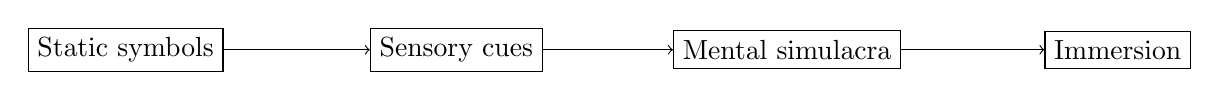
\begin{tikzpicture}
\node[draw, rectangle] (A) at (0,0) {Static symbols};
\node[draw, rectangle] (B) at (4.2,0) {Sensory cues};
\node[draw, rectangle] (C) at (8.4,0) {Mental simulacra};
\node[draw, rectangle] (D) at (12.6,0) {Immersion};
\draw[->] (A) -- (B);
\draw[->] (B) -- (C);
\draw[->] (C) -- (D);
\end{tikzpicture}
\end{figure}

This schematic is not a redraw of lecture art; it is a transcript-based compression of the lecture's central mechanism. Prose starts from marks on the page. If the language is chosen well, those marks activate the senses; the senses build an internal model; and the internal model becomes absorption.

\subsection{Question \& Answer}

\paragraph{Question.} If prose gives us only symbols, how does it create felt experience?

\paragraph{Answer.} By arranging those symbols so that they do not stop at conceptual recognition. They must awaken hearing, touch, motion, sight, smell, taste, and then bind these into a coherent imaginative state. Prose cannot show directly, so it must trigger indirectly.

\section{A Worked Reading of ``Ghost Quiet''}

Having established the general mechanism, the lecture turns to a single sentence and reads it with some care:
\[
\text{``The world was ghost quiet, except for the crack of sails and the burbling of water against hull.''}
\]
Before the sentence is analyzed, the lecturer names the main sensory field:
\begin{equation}
\{\text{taste},\ \text{smell},\ \text{touch},\ \text{hearing},\ \text{sight},\ \text{motion}\}.
\end{equation}
But this list is not the whole story, because fiction also works through abstraction and complex association. The power of the sentence comes from both.

We can reconstruct the lecturer's layered reading as follows:
\begin{align}
\text{description} &= \text{hearing} + \text{motion/touch} + \text{metaphoric association},\\
\text{hearing} &= \text{quiet} + \text{crack} + \text{burbling},\\
\text{motion/touch} &= \text{sails} + \text{water against hull},\\
\text{metaphoric association} &= \text{ghost}.
\end{align}
The first step is auditory. The lecturer explicitly notes that the sentence does not use a flat generic term such as ``sound.'' Instead it uses words with particular textures. ``Crack'' and ``burbling'' are not interchangeable with a generic acoustic label; each carries a distinct qualitative shape.

Then a second layer is added. The sails imply movement, and the water against the hull implies contact, pressure, and surface. The sentence has now passed beyond hearing alone. Finally, the word ``ghost'' modifies ``quiet'' and gives us an abstract relation that is still felt as part of the scene. The lecture's larger point may be written
\begin{equation}
\text{sensory engagement} + \text{abstract association} \to \text{richer description}.
\end{equation}

\paragraph{Worked example.} The analytic order is important:
\begin{enumerate}
\item We isolate the sound-words: ``quiet,'' ``crack,'' ``burbling.''
\item We note that these are specific qualities, not a generic category.
\item We then add motion and touch through sails and water against hull.
\item Only after that do we register the abstract link between quiet and ghost.
\item The final effect is cumulative rather than additive in the ordinary sense.
\end{enumerate}

\subsection{Question \& Answer}

\paragraph{Question.} How does one sentence accumulate multiple sensory and conceptual layers?

\paragraph{Answer.} Because the words are not all doing the same job. Some specify sound, some imply movement or contact, and some create nonliteral association. A strong sentence distributes its labor across several registers and lets those registers reinforce one another.

\section{Simile, Metaphor, and Readerly Distance}

The next move is subtle and decisive. The lecturer does not merely praise the phrase ``ghost quiet.'' She contrasts it with a nearby alternative: ``quiet as a ghost.'' The difference is not grammatical only. It is experiential:
\begin{align}
\text{quiet as a ghost} &\Rightarrow \text{greater distance},\\
\text{ghost quiet} &\Rightarrow \text{greater immediacy}.
\end{align}
We may compress the formal distinction like this:
\begin{align}
\text{simile} &\to \text{overt comparison},\\
\text{metaphor} &\to \text{implied comparison}.
\end{align}
The lecture's claim is local, not universal. It is not that metaphor always defeats simile. It is that here the simile would insert an extra interpretive layer. We would be told more explicitly how to compare. The metaphor instead lets the comparison happen inside the phrase itself, with less announcement and therefore less distance from the felt scene.

This is why the lecturer speaks of simile as inserting a distancing layer between reader and experience. A phrase can either move us toward the scene or make us stop to inspect the comparison from outside.

\subsection{Question \& Answer}

\paragraph{Question.} What does simile add, and what distance does it impose?

\paragraph{Answer.} Simile adds explicitness. It tells us openly that one thing is being compared with another. That explicitness can be useful, but in this example it weakens immediacy. ``Ghost quiet'' fuses the terms more tightly and leaves us closer to the experience itself.

\section{Against Clich\'e: Fresh Connotation and the Reader's Labor}

The lecture now shifts from the local contrast between simile and metaphor to a broader warning against clich\'e. Writers are always told to avoid overused images, and here the reason is made precise:
\begin{equation}
\text{overused image} \Rightarrow \text{low reader engagement}.
\end{equation}
An image such as ``red as a rose'' asks very little of us. The comparison arrives pre-consumed. The reader is not required to build much.

By contrast, a phrase such as ``stewed cherry dress'' produces a different kind of work:
\begin{equation}
\text{unexpected connotation} \to \text{reader participation} \to \text{immersion}.
\end{equation}
The reader has to infer the color, texture, density, even the social atmosphere that the phrase suggests. That inferential labor is not a defect. It is part of the pleasure. The reader meets the writer halfway and enters the scene by helping to construct it.

This is why the lecture ends where it does. We are told to use well-chosen words to engage sound, sight, taste, touch, smell, and movement, and then to create unexpected connotations among the elements of the story. The culminating prescription may be written as
\begin{equation}
\text{sense} + \text{fresh association} \Rightarrow \text{dynamic imaginative world}.
\end{equation}
The phrase about ``brushfire imaginations'' is not rhetoric added at the end for color. It is the logical terminus of the whole lecture. Description works when it ignites active imaginative response.

\section{Summary}

The lecture proceeds in a tight order. We begin with the reader's desire to be absorbed. We then ask what language must do if fiction is to satisfy that desire. A metaphorical description of Billy shows that vivid phrasing can move us closer to felt experience than flat summary can. From there we widen to a theory of prose as a medium of static symbols that must nevertheless construct sensation. The sentence about a world that was ``ghost quiet'' gives us a worked example of layered description: hearing, motion, touch, and abstraction in one compact unit. Finally, the lecture distinguishes metaphor from simile by the degree of distance each creates, warns against clich\'e, and argues that fresh connotation recruits the reader into the making of the scene. The final lesson is severe and simple: description is one of the places where fiction turns language into experience.